
\begin{figure}[H]
    \centering
    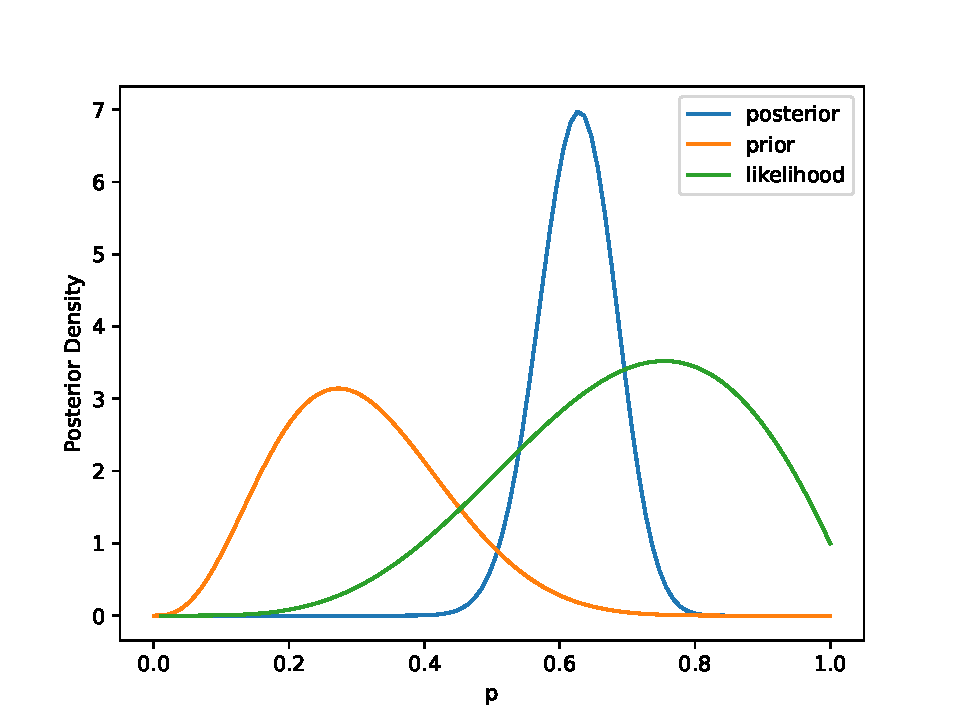
\includegraphics[width=0.8\linewidth]{images/new_bnb_posterior_density.pdf}
    \caption{Posterior density. Prior $B(a=4, b=9)$.}
    \label{fig:new-posterior}
\end{figure}

\begin{center}
    \begin{tabular}{rrrl}
\toprule
Posterior Mean & Posterior Mode & Posterior Median & Posterior Intervals (0.95) \\
\midrule
0.625 & 0.629 & 0.626 & 0.511, 0.732 \\
\bottomrule
\end{tabular}

\end{center}

Note that, although the choice of prior is radically different, the posterior (and its summaries) remain relative unchanged. The original posterior mode was slightly higher (0.695 vs. 0.629), which means that the new prior (whose center is much lower) affected our conclusion. To affect out conclusion more meaningfully, a different prior distribution would be necessary. 
